\documentclass[]{scrartcl}
\usepackage{graphicx}
\usepackage{geometry}
\geometry{
	a4paper,
	total={170mm,257mm},
	left=20mm,
	top=20mm,
}


%opening
\title{SDD -Hearts Low Level Design}
\author{Brandon Smith, Nieka Gutenberger, Joseph Coppin, Ryan Frazier, Trevor Jewkes}

\begin{document}

\maketitle
\pagebreak
	
	\noindent\makebox[\textwidth{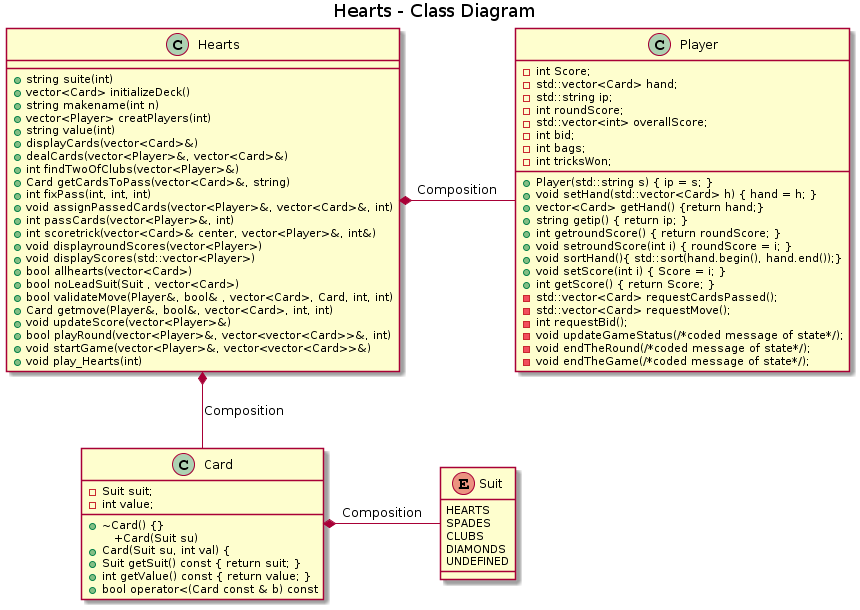
\includegraphics[width=\textwidth]{hearts.png}}]


\section{Hearts Class}


\subsection{string suite(int i)}  
	Converts enum of ints to string of card suit.
\subsection{vector $\langle$Card$\rangle$ initializeDeck()} \
	Creates deck of cards taken from card class.
\subsection{string makename(int n) } 
	Creates a player name.
\subsection{vector$\langle$Player$\rangle$  creatPlayers(int p) } 
	Creates a vector of Players to play the game.
\subsection{string value(int i)}
\subsection{void displayCards(vector$\langle$Card$\rangle$ \& hand)}
	Displays the deck for screen purposes.
\subsection{void dealCards(vector$\langle$Player$\rangle$ \& players, vector$\langle$Card$\rangle$ \& Deck)}
	Deals cards to players.
\subsection{int findTwoOfClubs(vector$\langle$Player$\rangle$ \& p)}  
	Looks through each hand to find the 2 of clubs to find starting player and hand.
\subsection{Card getCardsToPass(vector$\langle$Card$\rangle$ \& h, string p) }
	Gets and stores cards for passing at the beginning of each round.
\subsection{int fixPass(int r, int p, int c)}
	Ensures that cards are passed to the right players depending on the round.
\subsection{void assignPassedCards(vector$\langle$Player$\rangle$ \& p, vector$\langle$Card$\rangle$ \& h, int r)  }
	Takes the passed cards and redistributes based on round.
\subsection{int passCards(vector$\langle$Player$\rangle$ \& p, int round)  }
	Function for passing cards at beginging of round.
\subsection{int scoretrick(vector$\langle$Card$\rangle$ \& center, vector$\langle$Player$\rangle$ \& players, int\& turn)}
	Holds the score for the current trick.
\subsection{void displayroundScores(vector$\langle$Player$\rangle$ p)}
	Displays scores for the round.
\subsection{void displayScores(vector$\langle$Player$\rangle$  p)}
	Display scores each turn.
\subsection{bool allhearts(vector$\langle$Card$\rangle$ h)  }
	Checks to see if a players hand is all hearts.
\subsection{bool noLeadSuit(Suit s, vector$\langle$Card$\rangle$ h) }
	 cCmpares hand against the lead suit
\subsection{bool validateMove(Player\& p, bool\& broken, vector$\langle$Card$\rangle$  Center, Card move, int t, int i)}
\subsection{Card getmove(Player\& p, bool\& b, vector$\langle$Card$\rangle$  c, int t, int i)}
\subsection{void updateScore(vector$\langle$Player$\rangle$ \& p)}
	Adds round score to Score.
\subsection{bool playRound(vector$\langle$Player$\rangle$ \& players, vector$\langle$vector$\langle$Card$\rangle$ $\rangle$\& history, int round)}
\subsection{void startGame(vector$\langle$Player$\rangle$ \& players, vector$\langle$vector$\langle$Card$\rangle$ $\rangle$\& history) }
	 Uses players and calls round until game is over
\subsection{void play\_Hearts(int num)}



\end{document}
